% IEEE TPAMI version (IEEEtran, compsoc journal). Not compiled in this workspace: IEEEtran.cls
% ships with TeX Live full / Overleaf. IJCV: use Springer Nature's sn-jnl class with the same \input lines.
% A journal version of a conference paper needs substantial new material and a summary of changes.
\documentclass[10pt,journal,compsoc]{IEEEtran}
\usepackage[capitalize]{cleveref}
% Shared macros for the CV versions (CVPR/ICCV, ECCV, TPAMI/IJCV).
\usepackage{amsmath,amssymb}
\usepackage{graphicx}
\usepackage{booktabs}
\usepackage{multirow}
\usepackage{xcolor}
\usepackage{tikz}
\usetikzlibrary{positioning,arrows.meta,fit}
\usepackage{adjustbox}
% A table shrinks to the line width when it is wider, and is never enlarged
% (ECCV is one column, so \columnwidth there is the full text width).
\newcommand{\fittable}[1]{\adjustbox{max width=\linewidth}{\input{#1}}}
% Column gap of the full-width tables; a venue may set it before loading these macros.
\providecommand{\widetabcolsep}{4pt}
\providecommand{\todo}[1]{{\color{red}#1}}
\providecommand{\TODO}[1]{\textbf{\color{red}[TODO: #1]}}
\providecommand{\etal}{et al.\@}
\newcommand{\method}{KnotSight}            % working name of the system; change freely
\newcommand{\bench}{KnotBench-Photo}
\newcommand{\ou}{over/under}
\newcommand{\cw}{cable width}
% numbers are written by scripts/make_cv_tables.py into tables/numbers.tex
% generated by scripts/make_cv_tables.py -- do not edit
\newcommand{\BasePrec}{0.11}
\newcommand{\BaseRecall}{0.16}
\newcommand{\BaseOU}{0.49}
\newcommand{\BaseWrongNoGate}{10}
\newcommand{\VoneRecall}{0.90}
\newcommand{\VoneCov}{52}
\newcommand{\VoneUnseenCov}{31}
\newcommand{\VthreePrec}{0.93}
\newcommand{\VthreeRecall}{0.997}
\newcommand{\VthreeOU}{1.00}
\newcommand{\VthreeCov}{69}
\newcommand{\VthreeUnseenCov}{40}
\newcommand{\VthreeWrong}{0}
\newcommand{\VthreeImages}{240}
\newcommand{\VthreeCables}{60}
\newcommand{\SilOU}{0.62}
\newcommand{\SilCov}{0}
\newcommand{\CloseCovVone}{26}
\newcommand{\CloseCovVthree}{48}
\newcommand{\CloseLowVone}{0}
\newcommand{\CloseLowVthree}{8}
\newcommand{\CloseMidVone}{12}
\newcommand{\CloseMidVthree}{64}
\newcommand{\CloseWrong}{1}
\newcommand{\RealN}{166}
\newcommand{\RealAns}{12}
\newcommand{\RealWrong}{0}
\newcommand{\RealVoneAns}{5}
\newcommand{\RealPhotoN}{27}
\newcommand{\RealPhotoAns}{0}
\newcommand{\NoEulerWrong}{0}
\newcommand{\GzeroSilCov}{62}
\newcommand{\GzeroSilWrong}{25}
\newcommand{\NoTTASilCov}{12}
\newcommand{\NoTTASilWrong}{6}
\newcommand{\SeedCov}{68}
\newcommand{\SeedCovSd}{3}
\newcommand{\SeedUnseen}{37}
\newcommand{\SeedUnseenSd}{5}
\newcommand{\SeedWrong}{0}
\newcommand{\NoFFTCov}{63}
\newcommand{\NoFFTUnseen}{33}
\newcommand{\UPCov}{86}
\newcommand{\UPUnseenCov}{74}
\newcommand{\UPWrong}{0}
\newcommand{\UPBlindAns}{138}
\newcommand{\UPBlindCorrect}{129}
\newcommand{\UPBlindWrong}{9}
\newcommand{\UPBlindDrawAns}{94}
\newcommand{\UPBlindDrawWrong}{8}
\newcommand{\UPRealAns}{15}
\newcommand{\UPCloseCov}{50}
\newcommand{\USegRecall}{0.997}
\newcommand{\USegPrec}{0.99}
\newcommand{\BlindN}{308}
\newcommand{\BlindAns}{83}
\newcommand{\BlindCorrect}{78}
\newcommand{\BlindWrong}{5}
\newcommand{\BlindDrawN}{98}
\newcommand{\BlindDrawAns}{42}
\newcommand{\BlindDrawWrong}{5}
\newcommand{\BlindRendN}{210}
\newcommand{\BlindRendAns}{41}
\newcommand{\BlindRendWrong}{0}
\newcommand{\ClfBenchAcc}{12}
\newcommand{\ClfBlindAcc}{0.6}
\newcommand{\ClfTrainAcc}{18}
\newcommand{\PlainVtwoCorrect}{52.3}
\newcommand{\PlainVtwoMin}{51}
\newcommand{\PlainVtwoMax}{54}
\newcommand{\PlainRealMin}{11}
\newcommand{\PlainRealMax}{13}
\newcommand{\GapVtwoCorrect}{57}
\newcommand{\GapVtwoWrong}{1}
\newcommand{\FrozenVtwoCorrect}{54}
\newcommand{\FrozenVtwoWrong}{1}
\newcommand{\FrozenVtwoAns}{55}
\newcommand{\VtwoN}{312}
\newcommand{\VtwoDrawN}{105}
\newcommand{\VtwoRendN}{207}
\newcommand{\GapVtwoDrawCorrect}{30}
\newcommand{\FrozenVtwoDrawCorrect}{26}
\newcommand{\GapVoneCorrect}{84}
\newcommand{\GapVoneWrong}{6}
\newcommand{\UPVtwoAns}{96}
\newcommand{\UPVtwoCorrect}{95}
\newcommand{\UPVtwoWrong}{1}
\newcommand{\MkCpuUnseenDiffs}{+0, +15, +15}
\newcommand{\MkCpuUnseenMean}{+10.0}
\newcommand{\MkCpuUnseenPos}{2}
\newcommand{\MkCpuUnseenN}{3}
\newcommand{\MkCpuBenchDiffs}{+0, +8, +7}
\newcommand{\MkCpuBenchMean}{+5.0}
\newcommand{\MkCpuBenchPos}{2}
\newcommand{\MkCpuBenchN}{3}
\newcommand{\MkCpuVtwoDiffs}{+5, +1, +5}
\newcommand{\MkCpuVtwoMean}{+3.7}
\newcommand{\MkCpuVtwoPos}{3}
\newcommand{\MkCpuVtwoN}{3}
\newcommand{\MkCpuRealDiffs}{+5, -1, -1}
\newcommand{\MkCpuRealMean}{+1.0}
\newcommand{\MkCpuRealPos}{1}
\newcommand{\MkCpuRealN}{3}
\newcommand{\MkMpsUnseenDiffs}{+4, +8, +22}
\newcommand{\MkMpsUnseenMean}{+11.4}
\newcommand{\MkMpsUnseenPos}{3}
\newcommand{\MkMpsUnseenN}{3}
\newcommand{\MkMpsBenchDiffs}{+2, +4, +11}
\newcommand{\MkMpsBenchMean}{+5.7}
\newcommand{\MkMpsBenchPos}{3}
\newcommand{\MkMpsBenchN}{3}
\newcommand{\MkMpsVtwoDiffs}{+8, +6, +10}
\newcommand{\MkMpsVtwoMean}{+8.0}
\newcommand{\MkMpsVtwoPos}{3}
\newcommand{\MkMpsVtwoN}{3}
\newcommand{\MkMpsRealDiffs}{+3, -2, -2}
\newcommand{\MkMpsRealMean}{-0.3}
\newcommand{\MkMpsRealPos}{1}
\newcommand{\MkMpsRealN}{3}
\newcommand{\BiasMpsUnseenDiffs}{+9, +10, +17}
\newcommand{\BiasMpsUnseenMean}{+12.0}
\newcommand{\BiasMpsUnseenPos}{3}
\newcommand{\BiasMpsUnseenN}{3}
\newcommand{\BiasMpsBenchDiffs}{+5, +5, +8}
\newcommand{\BiasMpsBenchMean}{+5.8}
\newcommand{\BiasMpsBenchPos}{3}
\newcommand{\BiasMpsBenchN}{3}
\newcommand{\BiasMpsVtwoDiffs}{+6, +5, -2}
\newcommand{\BiasMpsVtwoMean}{+3.0}
\newcommand{\BiasMpsVtwoPos}{2}
\newcommand{\BiasMpsVtwoN}{3}
\newcommand{\BiasMpsRealDiffs}{+4, -1, -4}
\newcommand{\BiasMpsRealMean}{-0.3}
\newcommand{\BiasMpsRealPos}{1}
\newcommand{\BiasMpsRealN}{3}
\newcommand{\LebMpsUnseenDiffs}{-1, +12, +15}
\newcommand{\LebMpsUnseenMean}{+8.6}
\newcommand{\LebMpsUnseenPos}{2}
\newcommand{\LebMpsUnseenN}{3}
\newcommand{\LebMpsBenchDiffs}{-1, +6, +7}
\newcommand{\LebMpsBenchMean}{+3.9}
\newcommand{\LebMpsBenchPos}{2}
\newcommand{\LebMpsBenchN}{3}
\newcommand{\LebMpsVtwoDiffs}{+1, +1, +7}
\newcommand{\LebMpsVtwoMean}{+3.0}
\newcommand{\LebMpsVtwoPos}{3}
\newcommand{\LebMpsVtwoN}{3}
\newcommand{\LebMpsRealDiffs}{+1, +5, -2}
\newcommand{\LebMpsRealMean}{+1.3}
\newcommand{\LebMpsRealPos}{2}
\newcommand{\LebMpsRealN}{3}
\newcommand{\BiasCpuUnseenDiffs}{+3}
\newcommand{\BiasCpuUnseenMean}{+3.3}
\newcommand{\BiasCpuUnseenPos}{1}
\newcommand{\BiasCpuUnseenN}{1}
\newcommand{\BiasCpuBenchDiffs}{+1}
\newcommand{\BiasCpuBenchMean}{+0.8}
\newcommand{\BiasCpuBenchPos}{1}
\newcommand{\BiasCpuBenchN}{1}
\newcommand{\BiasCpuVtwoDiffs}{+6}
\newcommand{\BiasCpuVtwoMean}{+6.0}
\newcommand{\BiasCpuVtwoPos}{1}
\newcommand{\BiasCpuVtwoN}{1}
\newcommand{\BiasCpuRealDiffs}{+2}
\newcommand{\BiasCpuRealMean}{+2.0}
\newcommand{\BiasCpuRealPos}{1}
\newcommand{\BiasCpuRealN}{1}
\newcommand{\LebCpuUnseenDiffs}{-5}
\newcommand{\LebCpuUnseenMean}{-5.0}
\newcommand{\LebCpuUnseenPos}{0}
\newcommand{\LebCpuUnseenN}{1}
\newcommand{\LebCpuBenchDiffs}{-2}
\newcommand{\LebCpuBenchMean}{-2.5}
\newcommand{\LebCpuBenchPos}{0}
\newcommand{\LebCpuBenchN}{1}
\newcommand{\LebCpuVtwoDiffs}{+2}
\newcommand{\LebCpuVtwoMean}{+2.0}
\newcommand{\LebCpuVtwoPos}{1}
\newcommand{\LebCpuVtwoN}{1}
\newcommand{\LebCpuRealDiffs}{-4}
\newcommand{\LebCpuRealMean}{-4.0}
\newcommand{\LebCpuRealPos}{0}
\newcommand{\LebCpuRealN}{1}
\newcommand{\MkCpuN}{3}
\newcommand{\MkCpuBench}{72}
\newcommand{\MkCpuUnseen}{47}
\newcommand{\MkCpuVtwo}{56.0}
\newcommand{\UPUnseenCovExact}{74}
\newcommand{\BUUnetVtwo}{101.3}
\newcommand{\BUUfVtwo}{110.7}
\newcommand{\BUUnetReal}{19.3}
\newcommand{\BUUfReal}{25.3}
\newcommand{\BUUnetBench}{92.1}
\newcommand{\BUUfBench}{90.4}
\newcommand{\BUUnetUnseen}{85.8}
\newcommand{\BUUfUnseen}{82.5}
\newcommand{\BUUfVtwoDiffs}{+12, +9, +7}
\newcommand{\BUUfRealDiffs}{+4, +6, +8}
\newcommand{\BUUfUnseenDiffs}{-10.8, +1.7, -0.8}
\newcommand{\BUUnetVtwoWrong}{2}
\newcommand{\BUUfVtwoWrong}{3}
\newcommand{\BUUnetRealWrong}{2}
\newcommand{\BUUfRealWrong}{3}
\newcommand{\BUVtwoOnlyUf}{43}
\newcommand{\BUVtwoOnlyUnet}{15}
\newcommand{\BUVtwoSeedP}{0.02, 0.06, 0.12}
\newcommand{\BURealOnlyUf}{26}
\newcommand{\BURealOnlyUnet}{9}
\newcommand{\BURealSeedP}{0.51, 0.18, 0.04}
\newcommand{\BUNanoVtwo}{71.3}
\newcommand{\BUNanoUnseen}{72.8}
\newcommand{\BUTopoVtwo}{104.3}
\newcommand{\BUTopoUnseen}{84.7}
\newcommand{\BUTopoBench}{91.5}
\newcommand{\LearnedPmin}{1.89}
\newcommand{\LearnedPmax}{2.10}
\newcommand{\LearnedModels}{10}
\newcommand{\LearnedAlphaMin}{0.009}
\newcommand{\LearnedAlphaMax}{0.23}
\newcommand{\LearnedAlphaHeadMin}{0.18}
\newcommand{\LearnedAlphaHeadMax}{0.23}
\newcommand{\GapLambda}{1.7}
\newcommand{\GapTau}{0.4}
\newcommand{\GapDevAns}{136}
\newcommand{\GapDevWrong}{0}
\newcommand{\GapDevNoCheckAns}{135}
\newcommand{\GapDevCross}{856}
\newcommand{\GapDevNetWrong}{85}
\newcommand{\GapVetoAns}{131}
\newcommand{\GapLLnone}{-155}
\newcommand{\GapLLedge}{-151}
\newcommand{\GapLLxsec}{-142}


\usepackage{hyperref}
\begin{document}
\title{Read the Crossings, Compute the Knot: Knot Recognition from Images that Knows When to Abstain}
\author{Anonymous}
\IEEEtitleabstractindextext{%
% ---------------------------------------------------------------- abstract
\begin{abstract}
Recognising a knot in an image means reading a planar diagram (where the strands
cross and which strand is on top) and then computing its topology. Image-to-label
classifiers skip the diagram: they cannot name a knot outside their training census
and cannot say when an image does not show enough to decide. We split the problem.
A dense network predicts diagram structure (crossing centres, the over-strand axis,
cable masks and strand centre-lines); a geometric parser turns the maps into a
diagram, and exact knot invariants identify it. Checks that do not trust the network
(an Euler count of faces, a four-arm test at every crossing, agreement across
test-time views and across two centre-line resolutions) turn likely errors into
abstentions. The formulation is backbone-agnostic: with a pair of standard U-Nets it
answers \UPCov\% of photo-like images on \bench{} (\UPUnseenCov\% on unseen
backgrounds) with no wrong answer and abstains on every silhouette, where a 250-class
image classifier is right on \ClfBenchAcc\% and a segmentation network alone can name
nothing. On a blind set of \BlindN{} drawings and renders from sources never used
during development, scored once, it is right on \UPBlindCorrect{} images and wrong on
\UPBlindWrong{}; the errors are drawings whose under-strand gaps are one or two pixels
wide. A U-Net with a transformer bottleneck, trained on the same data, beats the U-Net pair on a
second blind set at every one of three seeds (\BUUfVtwo{} vs \BUUnetVtwo{} correct of 312, on average) and
on real pictures, with about as many wrong answers. We release the benchmark, the blind protocol, an annotation tool for real cable
photographs and all code.
\end{abstract}

\begin{IEEEkeywords}knot recognition, structured prediction, selective prediction, curvilinear structures, topology\end{IEEEkeywords}}
\maketitle
\IEEEdisplaynontitleabstractindextext
\begin{figure*}[t]
\centering
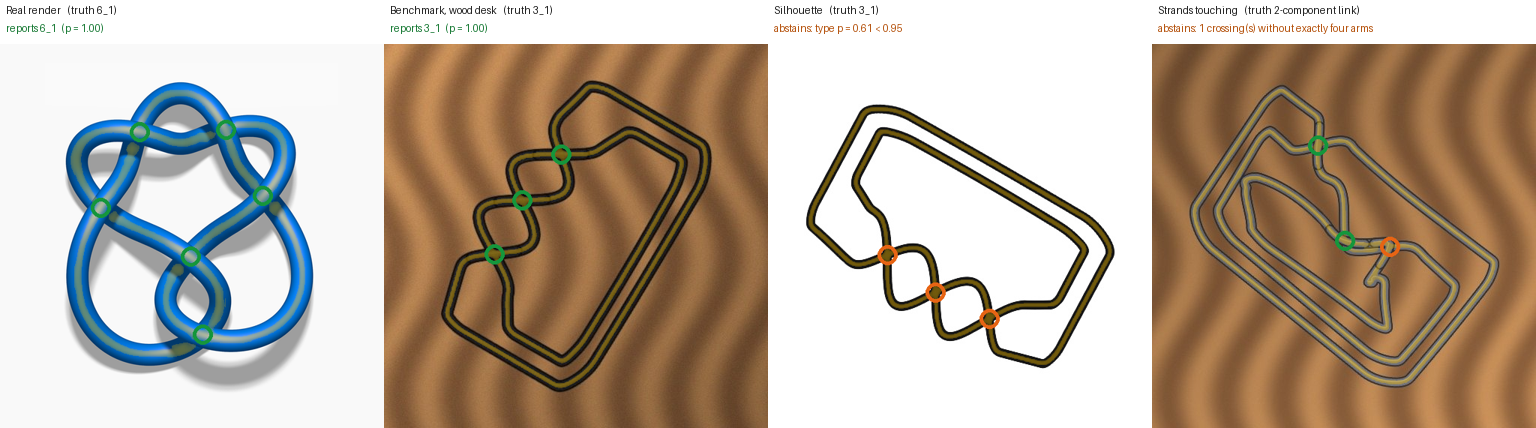
\includegraphics[width=\linewidth]{../figures/teaser.png}
\caption{\textbf{Read the diagram, compute the knot, abstain when the image is not
enough.} Green circles: crossings read with \ou{} probability $>0.9$; yellow: the
predicted strand centre-line. A real render and a benchmark cable are identified
exactly. On a silhouette the \ou{} reading disagrees across test-time views, so the
type probability stays below 0.95 and the system abstains. Where two strands touch, a
crossing loses an arm and the system abstains rather than guess.}
\label{fig:teaser}
\end{figure*}

% Shared body, included by every venue wrapper (cvpr/, eccv/, tpami/).
% ---------------------------------------------------------------- 1 introduction
\section{Introduction}\label{sec:intro}

A tangled cable, a surgical suture, a rope in a robot gripper, a knotted protein~\cite{taylor2000knotted} and a knot drawing in a
textbook pose the same question: \emph{which knot is this?} The answer is
topological and exact, but it has to be read from pixels. Two facts make the reading
hard. First, the decisive evidence is local and occluded: at each crossing one
strand passes over the other, and a single misread crossing can change the knot.
Second, many images do not contain the answer at all. A silhouette hides \ou{}, and two
strands that touch can hide a crossing. A useful system must therefore know when
not to answer.

Prior learned approaches predict a label from the whole image, such as a knot type from a fixed census or a crossing number~\cite{kauffman2022rectangular,dranowski2025knotdetection}.
Such a model cannot name a knot it was not trained on, cannot explain its answer
and returns a label even for a silhouette. Classical pipelines skeletonise the image
and search for junctions; on our benchmark the skeleton parser finds only
\BaseRecall{} of crossings and guesses \ou{} at chance (\BaseOU).

We instead \emph{learn perception and compute topology} (\cref{fig:teaser}). A dense
network predicts the parts a diagram is made of. A parser
assembles them into a planar diagram with geometric crossing signs, and exact
invariants (SnapPy, knot Floer homology) name the knot or link. The structure also
yields checks that do not trust the network. For a 4-valent planar projection the
number of enclosed faces equals crossings plus connected pieces, so a missed
crossing leaves an unexplained face. Every crossing must have four arms, the
\ou{} reading must agree across eight test-time views, and two centre-line
resolutions must give the same type. When a check fails, the system abstains and says
why.

\noindent Our contributions are:
\begin{enumerate}
\item A structured formulation of knot recognition from images: dense crossing,
  \ou{}, mask and centre-line maps, read into a diagram whose topology is computed
  exactly (\cref{sec:method}). It does not depend on the backbone: a 0.86M-parameter
  transformer and a pair of standard U-Nets both work, and the U-Nets are stronger
  (\UPCov\% vs \VthreeCov\% answered, \cref{tab:main}).
\item Consistency checks that convert errors into abstentions. Without test-time view
  agreement the model answers \NoTTASilCov\% of silhouettes, \NoTTASilWrong{} of them
  wrongly; the Euler gate removes all \BaseWrongNoGate{} wrong answers of a skeleton
  parser. With all checks our system gives \VthreeWrong{} wrong answers on
  \VthreeImages{} photo-like images and 60 silhouettes (\cref{sec:gates,tab:ablation}).
\item \bench{}: renders with exact ground truth, cable- and session-disjoint splits,
  topology accuracy with abstention and cable-level bootstrap intervals, plus a
  protocol and annotation tool for real cable photographs (\cref{sec:bench}).
\item An analysis of the main failure mode, strands passing within a \cw{}: a
  full-resolution centre-line head raises coverage at 1.0--1.3 \cw s from
  \CloseMidVone\% to \CloseMidVthree\%, and a first real-image test answers
  \RealAns{} of \RealN{} pictures with no error (\cref{sec:exp}).
\item A blind evaluation protocol: a frozen model, held-out sets frozen by hash, and a ledger
  that refuses to score a second main model. On \BlindN{} blind drawings and renders the
  system answers \BlindAns{} and errs on \BlindWrong{}; we analyse these failures.
\end{enumerate}

% Method overview (TikZ). Shared by all venue versions.
\begin{figure*}[t]
\centering
\resizebox{\linewidth}{!}{%
\begin{tikzpicture}[
  box/.style={draw, rounded corners=2pt, align=center, font=\small, minimum height=0.95cm, inner sep=3pt},
  head/.style={draw, rounded corners=2pt, align=center, font=\scriptsize, minimum width=2.1cm, minimum height=0.5cm, inner sep=2pt},
  gate/.style={draw, rounded corners=2pt, align=left, font=\scriptsize, fill=gray!8, inner sep=3pt},
  arr/.style={-{Latex[length=2mm]}, thick}]
\node[box] (img) {Image\\RGB + FFT channel};
\node[box, right=0.5cm of img] (enc) {Conv stem\\$16{\times}16$ tokens\\+ count token};
\node[box, right=0.5cm of enc] (tr) {4 transformer\\blocks\\(global attention)};
\node[box, right=0.5cm of tr] (dec) {U-Net decoder\\$128{\times}128$\\+ $256{\times}256$ branch};
\node[head, right=0.6cm of dec, yshift=1.5cm] (h1) {cable mask $m$};
\node[head, below=0.1cm of h1] (h2) {crossing heatmap $h$};
\node[head, below=0.1cm of h2] (h3) {over-strand axis $\mathbf{o}$};
\node[head, below=0.1cm of h3] (h4) {strand axis};
\node[head, below=0.1cm of h4] (h5) {centre-line ridges $c$};
\node[box, right=0.6cm of h3] (parse) {Parser\\peaks $\to$ ridge skeleton\\$\to$ arms $\to$ pairing\\$\to$ \ou{} $\to$ tracing};
\node[box, right=0.5cm of parse] (topo) {Diagram\\$\to$ PD code\\$\to$ exact invariants};
\node[gate, below=0.45cm of parse, xshift=1.4cm] (gates) {Gates: Euler count $\cdot$ four arms $\cdot$ closure\\$\cdot$ two ridges agree $\cdot$ type $p\ge0.95$ (8 views)};
\node[box, right=0.5cm of topo, fill=gray!8] (out) {Knot type\\or abstain\\with reason};
\draw[arr] (img) -- (enc); \draw[arr] (enc) -- (tr); \draw[arr] (tr) -- (dec);
\foreach \h in {h1,h2,h3,h4,h5} \draw[arr] (dec.east) -- (\h.west);
\foreach \h in {h1,h2,h3,h4,h5} \draw[arr] (\h.east) -- (parse.west);
\draw[arr] (parse) -- (topo); \draw[arr] (topo) -- (out);
\draw[arr, dashed] (gates.north) -- ++(0,0.2) -| (out.south);
\end{tikzpicture}}
\caption{\textbf{Learn perception, compute topology.} The network predicts the parts of a
diagram, not a label. A geometric parser assembles them, exact invariants identify the
knot, and checks that do not trust the network decide whether to answer.}
\label{fig:method}
\end{figure*}

% ---------------------------------------------------------------- 2 related work
\section{Related work}\label{sec:related}

\paragraph{Knots in images and in data.} Machine learning on knots has mostly used
symbolic inputs: invariants and diagram codes~\cite{davies2021advancing,davies2022signature},
with graph networks on diagrams~\cite{xu2019powerful}, and grid diagrams have been
classified with deep networks~\cite{kauffman2022rectangular}. Closest to us,
Dranowski \etal~\cite{dranowski2025knotdetection} predict crossing number from
knot pictures with CNNs and transformers. They propose reconstructing PD codes and
computing invariants as future work. We build that second stage: diagram
reconstruction with \ou{}, exact identification and abstention, evaluated with
cable-disjoint splits. Robotic rope manipulation reads rope state from images as
keypoints or traced paths for grasping and
untangling~\cite{nair2017rope,grannen2020untangling,viswanath2023handloom}, not as a
knot type. Exact identification uses SnapPy~\cite{snappy}, KnotInfo~\cite{knotinfo}
and knot Floer homology~\cite{ozsvath2004knotfloer}.

\paragraph{Curvilinear structure and line drawings.} Vessel, road and neurite
extraction recover thin structures and their connectivity~\cite{ronneberger2015unet,bastani2018roadtracer,shit2021cldice}.
Wireframe parsers predict junctions and line segments~\cite{huang2018wireframe,zhou2019lcnn}, and
technical-drawing vectorisation recovers strokes~\cite{egiazarian2020vectorization}.
None of these recovers which strand lies on top at a crossing, which is what makes a
diagram a knot.

\paragraph{Dense structured prediction.} Our crossing head follows centre-heatmap
detectors~\cite{zhou2019objects,newell2016hourglass} with a focal
loss~\cite{lin2017focal}, and our backbone uses transformer
blocks~\cite{dosovitskiy2021vit}. Foundation features~\cite{kirillov2023sam,oquab2024dinov2}
are a natural alternative backbone, which we leave as a baseline to add.

\paragraph{Selective prediction.} Abstaining classifiers trade coverage for
risk~\cite{geifman2017selective}, and calibration aligns confidence with
accuracy~\cite{guo2017calibration}. Our abstentions come mostly from consistency
checks grounded in planar topology, not from a learned confidence threshold.

% ---------------------------------------------------------------- 3 problem, 4 method
\section{From pixels to a knot diagram}\label{sec:method}

\paragraph{Diagram model.} A diagram is a set of closed strands (polylines in the
image plane) and crossings. Each crossing has two passages: an over-strand and an
under-strand. Its sign is the right-hand rule $\operatorname{sign}(\mathbf{t}_o\times\mathbf{t}_u)$
on the strand tangents, and the diagram's PD code follows by walking each strand.
Identification is then exact: a hyperbolic exterior is matched by an isometry
certificate, and knot Floer homology settles the remaining cases, including the
unknot and chirality. An image fixes the diagram only if every crossing is visible
and its \ou{} can be seen. A silhouette shows crossings but not \ou{}, so it fixes
the projection but not the knot.

\paragraph{Input.} The image is resized to $256\times256$ and given four channels:
RGB and an FFT-cleaned grey channel (mirror-padded homomorphic filtering, which
removes slow illumination, followed by Wiener shrinkage).

\paragraph{Networks.} Any network that outputs the maps below can be used. We study two.
(a) A NanoTransformer (0.86M parameters): a convolutional stem (stride 4) feeds a $16\times16$ token grid plus
one count token into four transformer blocks (width 128, 4 heads). Global attention
lets evidence from both sides of a crossing meet. A light U-Net decoder with
stride-4 and stride-2 skips returns to a $128\times128$ grid, where five heads predict
(\cref{fig:method}):
\begin{itemize}
\item a soft cable mask $m$ (fraction of each cell covered);
\item a crossing heatmap $h$, trained with a centre-point focal loss;
\item the over-strand axis $\mathbf{o}=(\cos2\alpha,\sin2\alpha)$ near each crossing;
\item the strand axis elsewhere, used to pair arms;
\item a centre-line ridge $c=\exp(-d^2/2\sigma^2)$, where $d$ is the distance to the
  nearest strand centre-line.
\end{itemize}
A full-resolution branch (input-level convolutions fused with the decoder) predicts
the same ridge on a $256\times256$ grid. On the coarse grid, two centre-lines one
\cw{} apart are only 1.5--3 cells apart and merge. Axial (doubled-angle) targets make
a strand and its reverse identical, which is all an image can show. Dihedral
augmentations transform the axial targets consistently. (b) A pair of standard U-Nets
(1.6M parameters each, 5 levels from $256^2$ to $16^2$): one predicts the mask and the
centre-lines, the other the crossing heatmap with the over-strand axis as a per-keypoint
attribute, as in CenterNet~\cite{zhou2019objects}. (c) A \emph{UNetFormer} (2.9M parameters), a single
network that predicts every map. It has a U-Net encoder and decoder with skip connections at all five
resolutions, as in (b), and four transformer blocks (width 192, 6 heads) with a count token on the
$16\times16$ grid at the bottleneck, as in TransUNet~\cite{chen2021transunet}. The transformer's output
is added back to the bottleneck through a zero-initialised projection, so training starts from a
plain U-Net.

\paragraph{Parser.} (i) Crossings are heatmap peaks above 0.35, refined to sub-cell
position. (ii) The skeleton is taken from the thresholded ridge. Specks below
$(0.6w)^2$ pixels are removed, where $w$ is the estimated \cw. Short gaps between
facing ends are bridged, and the skeleton is cut on a disc around each crossing,
leaving arcs whose ends are the crossing's arms. On cluttered backgrounds the networks draw short
centre-line pieces on background texture. Of 134 free ends that made the NanoTransformer abstain on
the benchmark's unseen backgrounds, 128 lay off the cable. A separate piece that carries no
detected crossing and is open (its skeleton has an end) cannot belong to a closed diagram, so it is
removed. Closed loops without crossings, such as an unknot or an unlinked component, are kept.
(iii) Of the three ways to split
four arms into two strands, we take the one whose strands run straightest. (iv) The
strand whose axis agrees best with $\mathbf{o}$ is on top. Its probability is
$p=\tfrac12+\big(\sigma(\kappa\,\Delta)-\tfrac12\big)\,\rho^{\gamma}$, where $\Delta$ is the
margin between the two strands, $\kappa$ is fitted on the training split, and $\rho$
is the mean resultant length of $\mathbf{o}$ across eight test-time views
($\gamma=2$, chosen on a development set). Where the views disagree, as on a
silhouette, $\rho\to0$ and $p\to\tfrac12$. (v) Tracing arcs through crossings yields
oriented strands and passages, i.e.\ a diagram.

\paragraph{Gap evidence (optional).} View agreement cannot detect \ou{} evidence that every
view misreads in the same way. The picture can be checked directly: the strand on top keeps
its outline through the crossing, and the strand underneath loses it. For each strand through a
crossing we sample, every half pixel of arc length $t$ in the 512-pixel image, the contrast
across both of its edges at $\pm w/2$ on the normal. The edge is \emph{missing} where this
contrast is below $\tau=\GapTau$ times its median on the free part of the strand. The strand's
interruption is a Lebesgue measure,
\[ G=\tfrac1w\,\big|\{t\in[-T,T]:\text{edge missing at }t\}\big|,\qquad T=\tfrac{w}{2\sin\theta}+w,\]
where $\theta$ is the crossing angle. $D=G_{\text{under}}-G_{\text{over}}$ is the picture's
evidence for the network's reading. It enters the log-odds,
$\operatorname{logit}p'=\operatorname{logit}p+\lambda D$, and the reading flips if
$p'<\tfrac12$. $\lambda=\GapLambda$ maximises the likelihood of \GapDevCross{} matched
crossings on development images; no test image is involved.

\paragraph{Minkowski attention and a Lebesgue loss.} We test three changes to the
NanoTransformer, each added to the previous one.
(1)~\emph{Lebesgue (layer-cake) loss.} The parser thresholds the mask at levels
$t\in[0.15,0.85]$ and the ridges at 0.5. By the layer-cake formula, the mean over
$t\sim U[a,b]$ of the area of $\{\hat p>t\}\triangle\{m>t\}$ equals
$\mathbb E\,|\mathrm{clip}(\hat p,a,b)-\mathrm{clip}(m,a,b)|/(b-a)$. We add this term with weight 1
for the mask ($[0.15,0.85]$) and both ridges ($[0.3,0.7]$). It penalises exactly the pixels
whose thresholded value depends on the level.
(2)~\emph{Minkowski position bias.} Each head adds $-\alpha_h\|\mathbf r_i-\mathbf r_j\|_{p_h}$ to
its logits, where $\mathbf r$ are token positions on the $16\times16$ grid. Both
$p_h=1+\operatorname{softplus}(\rho_h)$ (initially 2) and $\alpha_h$ (initially 0.2 down to 0.01
across heads) are learned per block. The $\ell_p$ distance is invariant under the eight flips and
quarter turns of the square, the group used for test-time views.
(3)~\emph{Minkowski content attention.} The logits are
$-t_h\|\mathbf q_i-\mathbf k_j\|_p^p/(p\sqrt d)$, with $p=1$ on two heads and $p=2$ on the other
two. For $p=2$ this is dot-product attention less a key-norm term. A learned $p$ would require
a per-coordinate $|\mathbf q-\mathbf k|^p$ tensor, about 400 times slower on a CPU.

\section{Consistency checks and abstention}\label{sec:gates}
The system reports a type only if all of the following hold; otherwise it abstains
and names the failed check.
\begin{enumerate}
\item \textbf{Euler count.} The projection of $k$ closed curves with $n$ crossings is a
  4-valent planar graph, so the ridge band has $n+\pi$ bounded faces, where $\pi$ is
  the number of connected pieces. A missed crossing adds an unexplained face.
\item \textbf{Four arms.} Every detected crossing has exactly four arms. No skeleton
  branch point lies away from a detected crossing.
\item \textbf{Closure.} The traversal closes. Free ends require a recorded closure
  (a fixture, or ends joined), as for open cables.
\item \textbf{Two resolutions agree.} The diagram is parsed from both ridges. If both
  pass, they must give the same type.
\item \textbf{Type probability.} Uncertain crossings are enumerated over their two
  readings, weighted by $p$, and the most likely type must reach probability 0.95.
\end{enumerate}

% ---------------------------------------------------------------- 5 benchmark
\section{\bench}\label{sec:bench}

\paragraph{Synthetic split.} Cables are random closed braids (2--4 strands, 2--9
generators) deformed in 3D and projected with a random rotation, so crossings, \ou{}
and the type are exact. They are rendered as shaded tubes in five sessions:
studio (S1), wood desk (S2), dim gradient (S3), cluttered texture (S4) and a
silhouette diagnostic (S0) where \ou{} is invisible. The benchmark has 300 images of
60 cables. S3 and S4 backgrounds never appear in training.

\paragraph{Splits and metrics.} Splits hold out whole cables and whole sessions;
views of one cable never straddle splits. We report:
\begin{itemize}
\item crossing precision and recall (Hungarian matching within one \cw);
\item \ou{} and pairing accuracy on matched crossings;
\item answered fraction and number of wrong answers (topology accuracy counts
  abstentions as wrong);
\item 95\% intervals from a bootstrap over cables.
\end{itemize}

\paragraph{Close-strands stress set.} The set has 100 renders binned by the smallest
centre-line gap between strand pieces away from crossings, in \cw s (0.6--1.0,
1.0--1.3, 1.3--1.7, $\ge$1.7), 25 per bin. It is used for development only; its
seeds are disjoint from training and the benchmark.

\paragraph{Real pictures.} 166 public images of knots (109 drawings, 22 3D renders,
8 logos and 27 photographs of physical objects), labelled only by knot type. The
measure is answered, correct (up to mirror image) or wrong.

\paragraph{Real cable photographs.} We provide a capture protocol and a browser
annotation tool. The protocol covers coax, rope and thread, four backgrounds, three
lights and three views per session. The tool records crossings with \ou{},
visibility, free ends and the closure. A scoring script evaluates them with the same
metrics after letterboxing, never stretching, the images.
\todo{Report the real cable set here once collected.}

% ---------------------------------------------------------------- 6 experiments
\section{Experiments}\label{sec:exp}

\paragraph{Training.} The model (0.86M parameters) is first trained on 2{,}000 tube renders
(plain and wood backgrounds only) for 14 epochs. It is then fine-tuned on 3{,}000
renders, 60\% of them in broader styles: outlined and hollow ribbons, textbook
diagrams with gaps, rope twist, shaded tubes, multicoloured links and widths of
5--32\,px. Torus, Lissajous and random Fourier curves are added to braid closures.
Finally the full-resolution ridge branch is trained for 4 epochs on the frozen
trunk. The full recipe takes about 2.5 hours on two CPU cores; we report three seeds.

\begin{table*}[t]
\centering\small
\setlength{\tabcolsep}{\widetabcolsep}
\fittable{../tables/main}
\caption{\textbf{Main results on \bench{}} (\VthreeImages{} photo-like images of
\VthreeCables{} cables; unseen = backgrounds S3/S4). Crossing precision (P) and recall (R),
\ou{} (O/U) accuracy on matched crossings, fraction of images answered, and wrong
answers. Our full model recovers \VthreeRecall{} of crossings and answers
\VthreeCov\% of images with \VthreeWrong{} wrong answers.}
\label{tab:main}
\end{table*}

\paragraph{Main results.} \Cref{tab:main} compares label prediction, a classical parser and
our formulation with three dense networks, all trained on the same renders. The 250-class
classifier has median top-class probability 0.007; forced to answer it is right on
\ClfBenchAcc\% of images, and at $p\ge0.95$ it answers none. The skeleton parser misses
most crossings and reads \ou{} at chance; without the Euler gate it gives
\BaseWrongNoGate{} wrong answers. A U-Net that only segments finds crossings as well as any
model (precision \USegPrec, recall \USegRecall) yet names nothing: without \ou{} evidence no
type reaches probability 0.95. Detecting crossings is not the hard part; reading \ou{} is.
With \ou{} heads, both backbones read crossings and \ou{} almost perfectly and make no wrong
call. The U-Net pair answers more (\UPCov\% vs \VthreeCov\%), most clearly on unseen
backgrounds (\UPUnseenCov\% vs \VthreeUnseenCov\%). It has 3.6 times the parameters and was
trained in one stage on the broader styles, while the NanoTransformer was first trained on
plain tube renders; a size-matched comparison is left open. Per-session results are in the
supplement.

\begin{table*}[t]
\centering\footnotesize
\setlength{\tabcolsep}{\widetabcolsep}
\fittable{../tables/beatunet}
\caption{\textbf{Matched comparison with the U-Net pair.} Same data (3{,}000 renders), same one-stage
recipe (12 epochs), same device (Apple GPU), and the same parser (with the clutter filter).
Mean$\pm$sd over three seeds; wrong answers are summed over seeds. Blind v2 has 312 images, real 166.}
\label{tab:beatunet}
\end{table*}

\paragraph{Beating the U-Net pair.} The U-Net pair's lead over the NanoTransformer does not come from
crossings or \ou{}, which both read almost perfectly on the benchmark. It comes from the dense path. On
cluttered backgrounds the NanoTransformer's centre-line and mask fire on background texture
(\cref{sec:method}). We therefore compare three models on equal terms (\cref{tab:beatunet}): the U-Net
pair, the NanoTransformer widened to the same size and trained in one stage, and the UNetFormer. The
widened NanoTransformer stays far behind (\BUNanoVtwo{} correct on blind v2), so size and training
recipe do not explain the gap. The UNetFormer answers more blind-v2 images correctly than the U-Net
pair at every seed (\BUUfVtwoDiffs; \BUUfVtwo{} vs \BUUnetVtwo{} on average). It also answers more real
pictures (\BUUfRealDiffs; \BUUfReal{} vs \BUUnetReal). Image by image, \BUVtwoOnlyUf{} blind-v2 readings
are correct only for the UNetFormer and \BUVtwoOnlyUnet{} only for the U-Net pair, summed over seeds
(exact McNemar $p=\BUVtwoSeedP$ per seed). On real pictures the split is \BURealOnlyUf{} vs
\BURealOnlyUnet. Wrong answers barely change: \BUUfVtwoWrong{} vs \BUUnetVtwoWrong{} on blind v2 over
three seeds, all of them the same drawing of 9\_25 read as 3\_1\,\#\,4\_1 by both models. On the
real pictures every error is on one picture, which the set holds twice: a single strand with three figure-eight lobes,
read as 4\_1\,\#\,4\_1\,\#\,4\_1 while its folder label is 4\_1. On the benchmark the U-Net pair keeps a
small edge (\BUUnetBench\% vs \BUUfBench\% answered, no wrong answer for either). On unseen
backgrounds the per-seed difference is \BUUfUnseenDiffs{} points. The clDice topology
loss~\cite{shit2021cldice} trades part of the UNetFormer's blind and real gain for benchmark coverage
(\BUTopoBench\%; \BUTopoVtwo{} correct on blind v2). The centre-line was not breaking, so a loss
against breaks was not the missing piece.

\begin{table}[t]
\centering\footnotesize
\setlength{\tabcolsep}{3pt}
\fittable{../tables/ablation}
\caption{\textbf{Ablations} on \bench{} (v3 trunk unless noted). Silh.\ ans.\ =
fraction of silhouettes answered, which must be 0 because \ou{} is not visible.}
\label{tab:ablation}
\end{table}

\paragraph{Ablations.} \Cref{tab:ablation} isolates the parser's components.
\begin{itemize}
\item \textbf{Skeleton source.} Coverage comes from the skeleton source. Mask, then
  128-grid ridge, then 256-grid ridge, then both ridges gives 52, 62, 68 and 69\%
  answered, and 31, 28, 39 and 40\% on unseen backgrounds.
\item \textbf{Test-time views.} Without them, the model answers \NoTTASilCov\% of
  silhouettes, \NoTTASilWrong{} of them wrongly: from one view it commits to an
  \ou{} reading it cannot see. Averaging the views without the consistency shrink
  ($\gamma=0$) is worse: \GzeroSilCov\% of silhouettes answered, \GzeroSilWrong{} wrongly.
  The shrink, not the averaging, is what makes the system abstain.
\item \textbf{FFT input channel and seeds.} Three seeds of the full recipe give
  \SeedCov$\pm$\SeedCovSd\% answered (\SeedUnseen$\pm$\SeedUnseenSd\% on unseen backgrounds) and
  \SeedWrong{} wrong answers in total. Retrained without the FFT channel (one seed) the model
  answers \NoFFTCov\% (\NoFFTUnseen\% unseen): slightly lower, but within about two standard
  deviations of the seed spread, so we do not claim a benefit from the channel.
\item \textbf{Clutter filter.} Removing open centre-line pieces that carry no crossing raises the frozen
  model's answered fraction from \VthreeCov\% to 82\% (unseen backgrounds 40\% to 68\%) and the CPU-trained
  U-Net pair's from 86\% to 92\%, with no new wrong answers. The filter was designed after inspecting the
  benchmark's unseen-background failures and checked on 80 new renders in those styles, so its benchmark
  gain is not blind. On blind v2 it changes the frozen model by 0 images and the U-Net pair by 1.
\item \textbf{Euler gate.} On renders the gate changes nothing for our model, since
  the other checks already catch its few misses. For the skeleton parser it removes
  all \BaseWrongNoGate{} wrong answers. We keep it as a network-independent safety
  net for real images, where detection is weaker.
\end{itemize}

\begin{figure}[t]
\centering
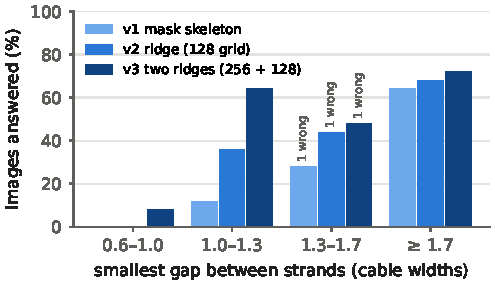
\includegraphics[width=\linewidth]{../figures/close_strands.pdf}
\caption{\textbf{Coverage as strands come closer} (100 images, 25 per bin). The
full-resolution centre-line head keeps strands apart down to about one \cw{}.
Below that, the strands touch and the system abstains. The single wrong answer
(same image in every version) is a 2.7\,px double crossing that no single view resolves.}
\label{fig:close}
\end{figure}

\paragraph{Strands that touch.} Abstentions on \bench{} come mostly from places where
two strands pass within a \cw{}. Their masks merge, the mask skeleton grows a false
branch, and the face between them disappears from the Euler count. Detection and
\ou{} are not the problem: crossing recall stays 0.93--0.97 and \ou{} accuracy
0.98--1.00 in every bin. \Cref{fig:close} shows that the
ridge skeleton raises overall coverage on the stress set from \CloseCovVone\% to
\CloseCovVthree\%. At 1.0--1.3 \cw s it rises from \CloseMidVone\% to \CloseMidVthree\%.
Below one \cw{} it reaches only \CloseLowVthree\%: there the strands touch, and
abstaining (and asking for another view) is the intended behaviour.

\begin{table}[t]
\centering\small
\setlength{\tabcolsep}{4pt}
\fittable{../tables/real}
\caption{\textbf{Real knot pictures answered} (166 public images, labelled by type
only); wrong answers in brackets. Traverser = skeleton parser.}
\label{tab:real}
\end{table}

\paragraph{Real pictures.} On 166 real knot pictures (\cref{tab:real}), the skeleton
parser answers none. Our model answers \RealVoneAns{} before and \RealAns{} after the
broader styles, all correct. Answers come from drawings and renders. None of the
\RealPhotoN{} photographs of physical objects (rope, cord, sculpture) is answered:
their textures still break the skeleton. The training styles were chosen after
inspecting four failures from this set, so these numbers are not a blind test.
\todo{Add a blind real set and the annotated real cable photographs.}

\begin{table}[t]
\centering\footnotesize
\setlength{\tabcolsep}{3pt}
\fittable{../tables/blind}
\caption{\textbf{Blind set}, scored once with the frozen model (\BlindN{} images from sources
never used or viewed during development: knotR drawings and POV-Ray renders of KnotPlot
centrelines). Correct = same type up to mirror image.}
\label{tab:blind}
\end{table}

\paragraph{Blind evaluation.} Before scoring, the NanoTransformer and its parser settings were
frozen by hash, and the set was built without viewing any image (\cref{tab:blind}). Renders behave like
the benchmark: \BlindRendAns{} of \BlindRendN{} answered, \BlindRendWrong{} wrong. Drawings expose a
failure mode the benchmark never showed: \BlindDrawAns{} of \BlindDrawN{} answered and
\BlindDrawWrong{} wrong (\cref{fig:blindfail}). In each of them the under-strand gap is one or two
pixels wide, every crossing is read with probability 0.96--0.99, and all eight test-time views agree
on the reading. View agreement detects evidence that depends on the view (a silhouette), not
evidence that is consistently misread. A network-independent check of the intensity break at each
crossing is the obvious next gate; it must be evaluated on a new blind set.

\begin{figure*}[t]
\centering
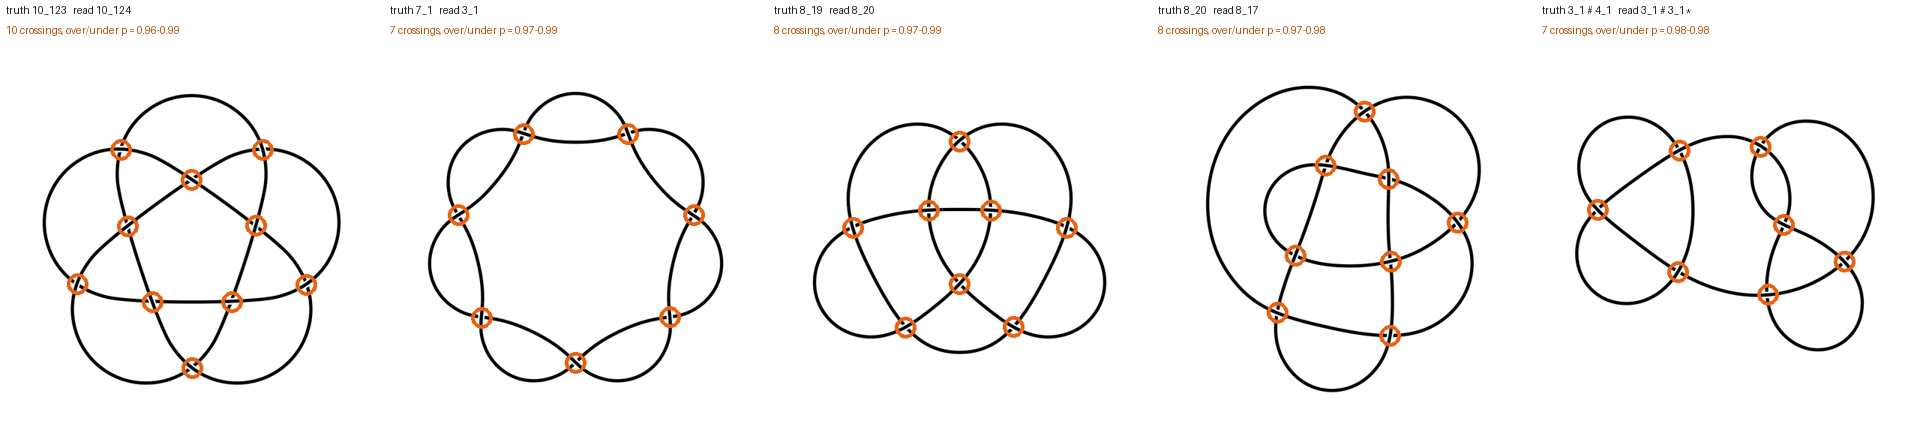
\includegraphics[width=\linewidth]{../figures/blind_failures.png}
\caption{\textbf{All wrong answers on the blind set} (post-scoring analysis). Orange circles: detected
crossings. Gaps at the under-strands are one or two pixels wide; the model reads \ou{} with
probability 0.96--0.99 at every crossing and all test-time views agree.}
\label{fig:blindfail}
\end{figure*}

\paragraph{Baselines on the blind set.} The U-Net pair, scored once as a baseline, answers
\UPBlindAns{} images, \UPBlindCorrect{} correctly; \UPBlindWrong{} of its answers are wrong,
\UPBlindDrawWrong{} of them on drawings with nearly invisible gaps, the same failure as the
frozen model. The classifier is right on \ClfBlindAcc\% of the blind set (and on \ClfTrainAcc\%
of the real pictures it was trained on).

\begin{table*}[t]
\centering\footnotesize
\setlength{\tabcolsep}{\widetabcolsep}
\fittable{../tables/minkowski}
\caption{\textbf{Minkowski attention, the Lebesgue loss and gap evidence.} Mean$\pm$sd over seeds;
wrong answers are summed over seeds. Variants are added cumulatively (\cref{sec:method}). A seed
fixes the data order and augmentation, so each variant has a plain counterpart with the same seed
(see text). $^\dagger$Blind v1 is no longer blind for the gap evidence, whose design followed its
errors. Blind v2 is (\cref{tab:blind2}).}
\label{tab:minkowski}
\end{table*}

\paragraph{Minkowski attention and the Lebesgue loss.} Each variant was trained with the full recipe
(\cref{tab:minkowski}). The content-attention variant has three CPU seeds: 0 and 1 on the machine that
trained the plain model, and 2 on a laptop CPU. All three variants also have three seeds trained on
an Apple GPU. A seed fixes the data order and augmentation, so we compare each variant with the
plain model of the same seed. Against it, Minkowski content attention changes the answered fraction
on unseen backgrounds by \MkCpuUnseenDiffs{} points on CPU, and the number of correct blind-v2
images by \MkCpuVtwoDiffs{}. It makes one more wrong blind-v2 answer over the three seeds (3 vs 2).
No paired comparison goes the other way. On the GPU the
differences are larger (\MkMpsUnseenDiffs{} points; \MkMpsVtwoDiffs{} images). However, the plain
model was never trained on the GPU, and the Lebesgue loss alone, which has no Minkowski component,
gains about as much there (\LebMpsUnseenDiffs{} points). The GPU rows therefore mix the device with the
model. On CPU at seed 0, the Lebesgue loss alone loses 5 points on unseen backgrounds and the
position bias gains 3. On the 166 real pictures there is no consistent change (\MkCpuRealDiffs{}).
No model makes a wrong benchmark call. On the close-strands set the variant makes 4 wrong answers over
three seeds, against 3 for the plain model. The learned exponents
stay Euclidean: $p\in[\LearnedPmin,\LearnedPmax]$ in every head of all \LearnedModels{} trained
models, and the slopes stay near their initial values (\LearnedAlphaMin--\LearnedAlphaMax). Whatever
helps is a multi-scale locality prior on the token grid, not a non-Euclidean neighbourhood. Seeds
alone move blind-v2 by up to three images (\PlainVtwoMin--\PlainVtwoMax{} correct for the plain
model). Three paired seeds give a consistent direction (benchmark coverage and blind v2 up, wrong
answers unchanged), not a precise effect size. The variants stay well behind the U-Net pair.

\begin{table}[t]
\centering\footnotesize
\setlength{\tabcolsep}{3pt}
\fittable{../tables/blind2}
\caption{\textbf{Blind set v2} (\VtwoN{} images, frozen before any model or setting in this
table was scored on it, never viewed: \VtwoDrawN{} line drawings with halo gaps of 0.1--0.8 line
widths, \VtwoRendN{} POV-Ray renders from new viewpoints). Correct = same type up to mirror image.}
\label{tab:blind2}
\end{table}

\paragraph{Gap evidence and a second blind set.} Blind v1 can no longer test a remedy for its own
failures, because they were inspected. We therefore froze a second blind set
(\cref{tab:blind2}) before scoring the gap evidence or any new model on it. Its drawings come
from a renderer used nowhere in training, with gaps from clear to nearly invisible. Its renders
show the v1 curves from new directions, which gives new diagrams. The three plain seeds answer
\PlainVtwoMin--\PlainVtwoMax{} images correctly (mean \PlainVtwoCorrect). With the gap evidence,
the frozen network answers \GapVtwoCorrect{} correctly (\FrozenVtwoCorrect{} without it) with
\GapVtwoWrong{} wrong answer, as before. The gain comes from drawings (\FrozenVtwoDrawCorrect{}
$\to$ \GapVtwoDrawCorrect{} correct). On the benchmark, the close-strands set and the real pictures,
nothing changes (\cref{tab:minkowski}). On development images the evidence improves the
log-likelihood of the network's \ou{} readings from \GapLLnone{} to \GapLLedge{} and adds one
answer (\GapDevNoCheckAns{} $\to$ \GapDevAns{}, no wrong). A veto rule ($p\to\frac12$ when $D$ is
small) instead removes correct answers (\GapVetoAns{} answered) and was not adopted.

Two caveats. First, a cross-section measure (correlation of the strand's profile with its free
profile) fits the development crossings better (log-likelihood \GapLLxsec). But on the shaded 3D
renders of the real-picture set it has the wrong sign at most crossings the network reads correctly
(all seven on one 7\_1 render), and it cost six correct answers there. We chose the edge measure after seeing this, so the
real-picture numbers for the gap evidence are not blind. Blind v2 was frozen before that choice
was scored. Second, the effect is small: three answers out of \VtwoN{}, just above the
seed-to-seed range. On blind v1 (post hoc) the evidence adds six correct answers and one
wrong, and the original five errors remain: they are not \ou{} errors alone, as 7\_1 read as
3\_1 shows. The U-Net pair is far stronger on v2 (\UPVtwoCorrect{} correct of \UPVtwoAns{}
answered, \UPVtwoWrong{} wrong), as on every other set.

\paragraph{Runtime.} On four CPU threads of a laptop (Apple silicon, PyTorch on CPU), the median
image takes 0.54\,s in the network with eight test-time views (0.08\,s with one) and 0.35\,s in the
parser, including both skeleton sources and the gap measure: 0.9\,s in total (20 benchmark images).

\begin{figure*}[t]
\centering
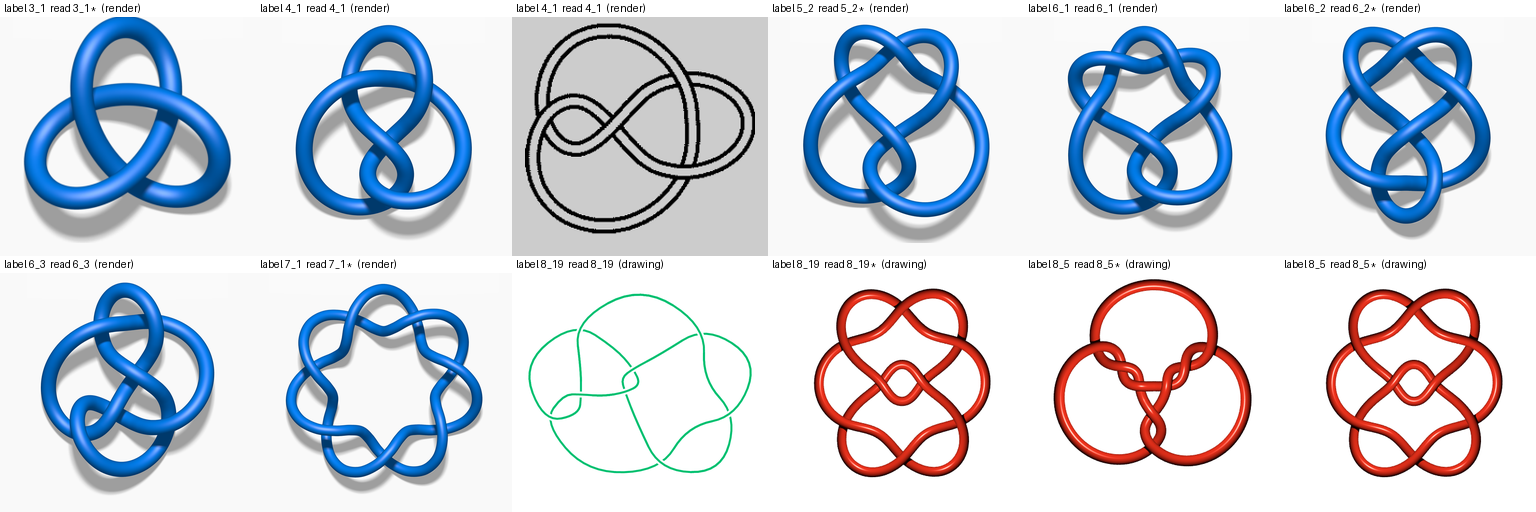
\includegraphics[width=\linewidth]{../figures/real_answered.png}
\caption{\textbf{All \RealAns{} real pictures our system answers}, each correct (up to
mirror image, marked $*$). Every answer comes from a drawing or a render; none of the
photographs of physical objects is answered.}
\label{fig:real}
\end{figure*}

% ---------------------------------------------------------------- 7 limitations, conclusion
\section{Limitations}\label{sec:limits}
Both backbones make confident errors on the blind set (\BlindWrong{} and \UPBlindWrong{}), almost
all on drawings with nearly invisible gaps: confidence is calibrated against view-dependent
ambiguity, not against consistent misreading. The picture's own gap evidence adds answers on a
second blind set without adding errors, but it does not remove those errors. The Minkowski
variants rest on three paired seeds per device, and the plain model was not trained on the GPU,
so their effect size is uncertain. All quantitative cable results are on renders. No annotated photographs of real cables
exist yet. On public pictures the system answers drawings and renders but no photograph
of a physical object, and those pictures informed our choice of training styles. Strands
that touch (gap below one \cw) and double crossings smaller than a few pixels
cannot be resolved from one view; multi-view fusion is implemented but untested on real
data. The output is a knot type, not a physical untangling plan: friction, stiffness
and tension decide how hard a cable is to undo.

\section{Conclusion}\label{sec:concl}
Reading the diagram and computing the topology, instead of classifying the image,
gives a knot recogniser that generalises past a census, explains its answers and
abstains when the image is not enough. The gain comes from the formulation, not from a
particular backbone: standard U-Nets do better than our first transformer, and a U-Net with a
transformer bottleneck does better than both on blind and real pictures. On renders it reads crossings and \ou{} almost
perfectly and makes no wrong call. The open problem is perception on real photographs,
for which we release the benchmark protocol, annotation tool and scoring code.


% journal-only material: full supplement in the paper body
% ---------------------------------------------------------------- supplementary material
\section*{Supplementary material}
\setcounter{section}{0}\renewcommand{\thesection}{S\arabic{section}}
\section{Per-session results}
\begin{table}[h]\centering\small\begin{tabular}{@{}lccccc@{}}
\toprule
Session & P & R & O/U & Answered & Wrong \\
\midrule
S1 studio (seen) & 1.00 & 1.00 & 1.00 & 98\% & 0 \\
S2 wood desk (seen) & 1.00 & 1.00 & 1.00 & 97\% & 0 \\
S3 dim (unseen) & 1.00 & 1.00 & 1.00 & 65\% & 0 \\
S4 clutter (unseen) & 0.77 & 1.00 & 1.00 & 15\% & 0 \\
S0 silhouette & 1.00 & 1.00 & 0.62 & 0\% & 0 \\
\bottomrule
\end{tabular}

\caption{\bench{} by session, full model.}\label{tab:sessions}\end{table}
\section{Close-strands stress set}
\begin{table}[h]\centering\small\begin{tabular}{@{}lccc@{}}
\toprule
Gap (\cw s) & v1 & v2 & v3 \\
\midrule
0.6--1.0 & 0\% & 0\% & 8\% \\
1.0--1.3 & 12\% & 36\% & 64\% \\
1.3--1.7 & 28\% (1) & 44\% (1) & 48\% (1) \\
$\ge$1.7 & 64\% & 68\% & 72\% \\
all 100 & 26\% (1) & 37\% (1) & 48\% (1) \\
\bottomrule
\end{tabular}

\caption{Answered fraction by gap; wrong answers in brackets.}\label{tab:close}\end{table}
\section{Rendering styles and training details}\todo{Style examples, hyper-parameters, augmentations.}
\section{Annotation tool and real-photo protocol}\todo{Screenshot, record schema, capture grid.}
\section{Symbolic knot benchmark}\todo{Optional: KnotBench invariant-learning results (Tasks 1--3) as motivation.}

\bibliographystyle{IEEEtran}
\bibliography{../references}
\end{document}
